\documentclass[12pt, a4paper]{report}
\usepackage[utf8]{inputenc}
\usepackage[T1]{fontenc}
\usepackage[utf8]{inputenc}
\usepackage{geometry}
\usepackage{listings}
\usepackage{xcolor}
\usepackage[]{graphicx}
\usepackage[export]{adjustbox}
\usepackage{subcaption}
\makeatletter
\setlength{\@fptop}{0pt}
\makeatother

\definecolor{codegreen}{rgb}{0.26, 0.61, 0}
\definecolor{codegray}{rgb}{0.5,0.5,5}
\definecolor{codepurple}{rgb}{58,0,0.82}
\definecolor{backcolour}{rgb}{0.80, 0.81, 0.93}

\lstdefinestyle{mystyle}{
    backgroundcolor=\color{backcolour},   
    commentstyle=\color{codegreen},
    keywordstyle=\color{magenta},
    numberstyle=\tiny\color{codegray},
    stringstyle=\color{codepurple},
    basicstyle=\ttfamily\footnotesize,
    breakatwhitespace=false,         
    breaklines=true,                 
    captionpos=b,                    
    keepspaces=true,                 
    numbers=left,                    
    numbersep=5pt,                  
    showspaces=false,                
    showstringspaces=false,
    showtabs=false,                  
    tabsize=2
}

\lstset{style=mystyle}


\title{\textbf{EE2703: Applied Programming Lab\\Assignment 8\\The Digital Fourier Transform
}}


\author{Devaganthan S S\\ EE19B018}
\date{\today}
\begin{document}

\maketitle


\section{Abstract}
The assignment aims to understand how DFT can be visualized in python using the fast Fourier algorithm

\section{Introduction}
In this assignment, we compute the DFT of Various Discrete-Time Signals using the function \textbf{fft()} from NumPy. We then visualize the DFTs after making certain modifications to the output of the \textbf{fft()} function. 
\section{Results and Implementation}
\subsection{Examples }
The range for the time axis is from -4$\pi$ to 4$\pi$ and the frequency range is from -64 to 64 with N = 512. The function \textbf{fftshift()} is used to get the desired spectrum. The below function plots the DFT spectrum of an array passed through it.
\noindent
\lstinputlisting[language = python]{code1.py}
\begin{figure}[h!]
    \centering
    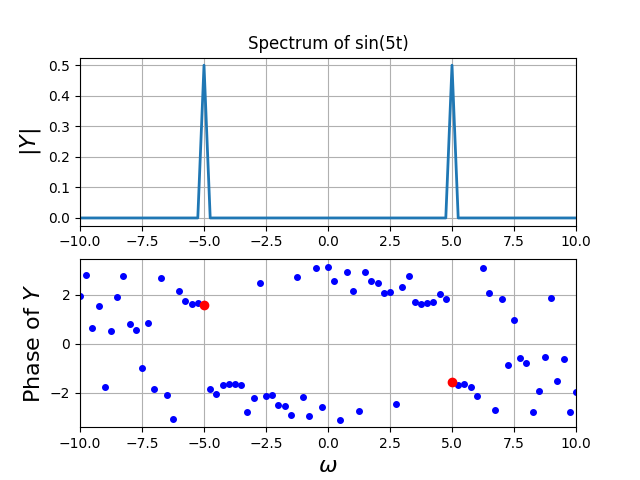
\includegraphics[scale=0.7]{fig1.png} 
    \caption{}
    \label{fig:my_label}
\end{figure}
\begin{figure}[h!]
    \centering
    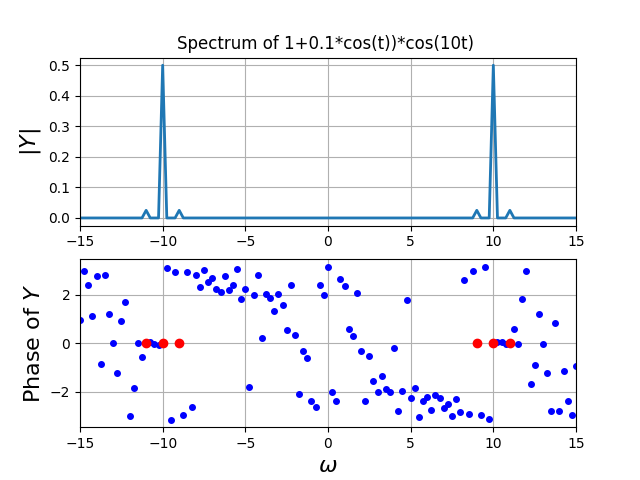
\includegraphics[scale=0.7]{fig2.png} 
    \caption{}
    \label{fig:my_label}
\end{figure}


\subsection{The spectrum of sin$^3$t and cos$^3$t:}
Using the same function as before, we get the below plot
\begin{figure}[h!]
    \centering
    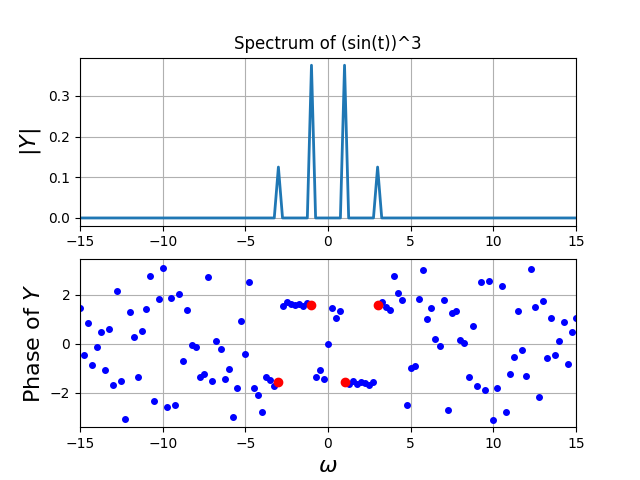
\includegraphics[scale=0.7]{fig3.png} 
    \caption{}
    \label{fig:my_label}
\end{figure}
\begin{figure}[h!]
    \centering
    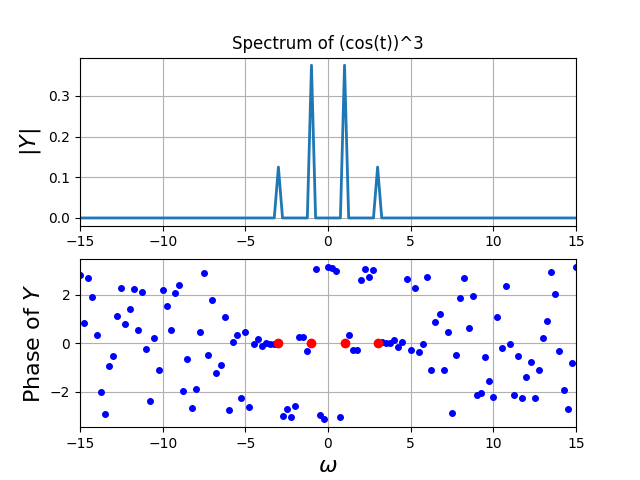
\includegraphics[scale=0.7]{fig4.png} 
    \caption{}
    \label{fig:my_label}
\end{figure}
\vspace{100mm}
\subsection{The spectrum of cos(20t+5 cos(t))}
Using the same function as before, we get the below plot
\noindent
\begin{figure}[h!]
    \centering
    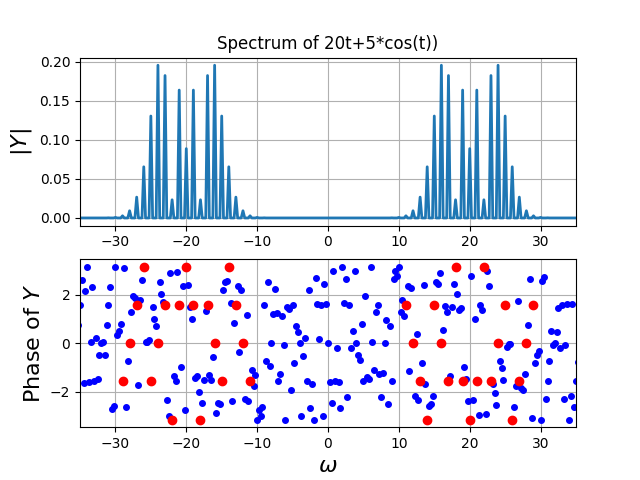
\includegraphics[scale=0.75]{fig5.png} 
    \caption{}
    \label{fig:my_label}
\end{figure}
\subsection{The spectrum of the Gaussian }
To get an error of less than 10$^-^6$, the range required is from -4$\pi$ to 4$\pi$. The below code finds the desired range for the gaussian and plots the spectrum for the same. The code finds the least square Error, from using the DFTs found using \textbf{fft()} function and the computed DFT.
\noindent
\lstinputlisting[language = python]{code2.py}
\begin{figure}[h!]
    \centering
    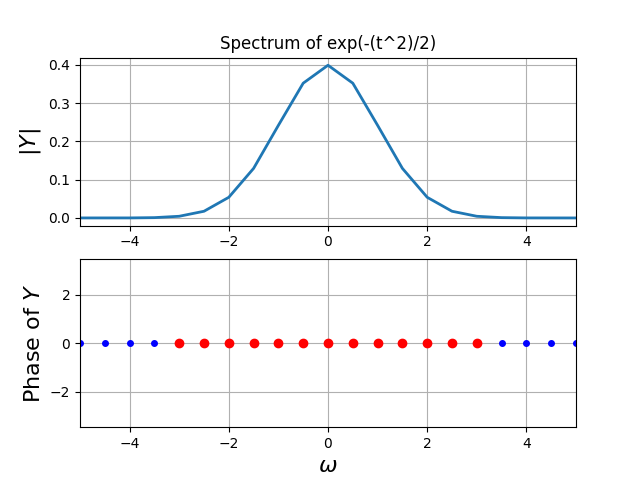
\includegraphics[scale=0.7]{fig6.png} 
    \caption{}
    \label{fig:my_label}
\end{figure}

\section{Conclusion}
With the help of the functions \textbf{fft()} and \textbf{fftshift()}, DFTs of time signals can be visualized in Python


\end{document}

